\begin{figure}[H]
\centering
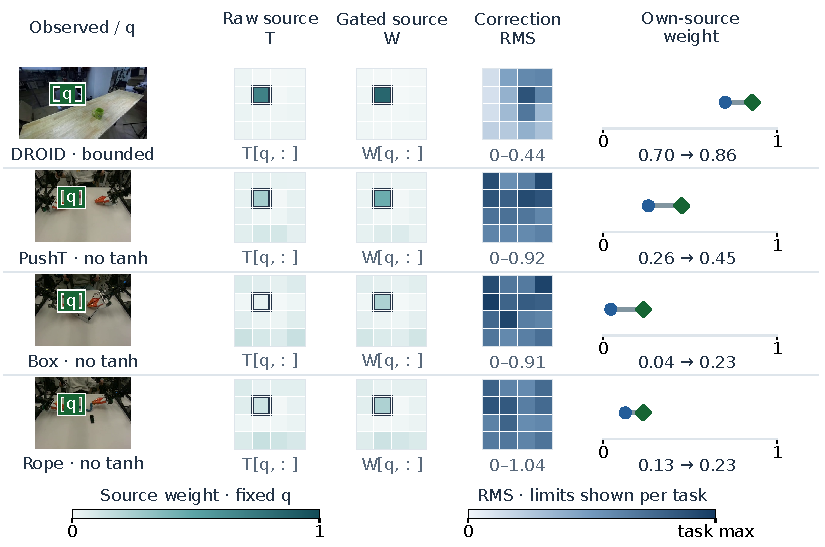
\includegraphics[width=\linewidth]{generated/qualitative_closest_v1/decoder_internals.pdf}
\caption{\textbf{A measured decoder view: read, retain and correct.}
Each row uses the middle-ranked trajectory's fixed window (DROID: 71st of 141;
IWS: fifth of ten, in decreasing-gain order). DROID uses bounded
ShiftWM; reserved IWS uses its no-$\tanh$ ablation. Weights and corrections
are at DROID $h=10$ and IWS offset 59 ($H=60$).
The outlined coordinate $q$ is always row 2, column 2 of the feature grid,
not an object localization. Maps $T[q,:]$ and $W[q,:]$
show all 16 observed-source weights for that destination patch, averaged over
three seeds on a common $[0,1]$ scale. Right: the same-location weight before
(circle) and after (diamond) gating. This increase follows algebraically from
$W=I-D+DT$ and does not establish an accuracy gain. Correction maps show the
mean of per-seed channel RMS values, with separate task scales printed below.
These are feature-mixing diagnostics, not semantic attention or physical motion.
Recorded scenes: DROID (CC BY 4.0) and RLA-WM/IWS.}
\label{fig:closest-decoder-internals}
\end{figure}
